%%
%%
%%   This file is part of the APS files in the REVTeX 4 distribution.
%%   Version 4.1r of REVTeX, August 2010
%%
%%
%%   Copyright (c) 2001, 2009, 2010 The American Physical Society.
%%
%%   See the REVTeX 4 README file for restrictions and more information.
%%
%
% This is a template for producing manuscripts for use with REVTEX 4.0
% Copy this file to another name and then work on that file.\label{\label{\part{\part{key}}}}
% That way, you always have this original template file to use.
%
% Group addresses by affiliation; use superscriptaddress for long
% author lists, or if there are many overlapping affiliations.
% For Phys. Rev. appearance, change preprint to twocolumn.
% Choose pra, prb, prc, prd, pre, prl, prstab, prstper, or rmp for journal
%  Add 'draft' option to mark overfull boxes with black boxes
%  Add 'showpacs' option to make PACS codes appear
%  Add 'showkeys' option to make keywords appear
%\documentclass[aps,pre,preprint,groupedaddress]{revtex4-1}
%\documentclass[aps,pre,preprint,superscriptaddress]{revtex4-1}
\documentclass[aps,pre,reprint,groupedaddress]{revtex4-1}

%\usepackage{silence}
%\WarningFilter{revtex4-1}{Repair the float}

\usepackage{amssymb}
\usepackage{amsmath}
\usepackage{amsfonts}
\usepackage{graphicx}
\usepackage{soul}
\usepackage{float}





%%%%%%%%%%%%%%%%%%%%%%%%%%%%%%%%%%%%%%%%%%%%%%%%%%%%%
%%%%% For colored text
\usepackage{color}
\newcommand{\red}[1]{\textbf{\textcolor{red}{(#1)}}}
\newcommand{\nk}[1]{\textcolor{magenta}{#1}}
%%%%%%%%%%%%%%%%%%%%%%%%%%%%%%%%%%%%%%%%%%%%%%%%%%%%%


% You should use BibTeX and apsrev.bst for references
% Choosing a journal automatically selects the correct APS
% BibTeX style file (bst file), so only uncomment the line
% below if necessary.
\bibliographystyle{apsrev4-1}

\makeatletter
\newcommand{\rmnum}[1]{\romannumeral #1}
\newcommand{\Rmnum}[1]{\expandafter\@slowromancap\romannumeral #1@}
\makeatother


\begin{document}

% Use the \preprint command to place your local institutional report
% number in the upper righthand corner of the title page in preprint mode.
% Multiple \preprint commands are allowed.
% Use the 'preprintnumbers' class option to override journal defaults
% to display numbers if necessary
%\preprint{}

%Title of paper
\title{Chaos synchronization in three coupled SQUIDs}

% repeat the \author .. \affiliation  etc. as needed
% \email, \thanks, \homepage, \altaffiliation all apply to the current
% author. Explanatory text should go in the []'s, actual e-mail
% address or url should go in the {}'s for \email and \homepage.
% Please use the appropriate macro foreach each type of information

% \affiliation command applies to all authors since the last
% \affiliation command. The \affiliation command should follow the
% other information
% \affiliation can be followed by \email, \homepage, \thanks as well.
\author{Joniald Shena}
\email[]{jonialdshena@misis.ru}
\affiliation{National University of Science and Technology MISiS, Leninsky prosp. 4, Moscow, 119049, Russia}
%\affiliation{Department of Mathematics, School of Science and Technology,
%Nazarbayev University, Astana, Republic of Kazakhstan}
\author{N. Lazarides}
\affiliation{Department of Physics, University of Crete, 71003 Heraklion, Greece }
\author{J. Hizanidis}
\affiliation{Department of Physics, University of Crete, 71003 Heraklion, Greece }
%\affiliation{Bradley Department of Electrical and Computer Engineering}
%\thanks{}
%\altaffiliation{}

%Collaboration name if desired (requires use of superscriptaddress
%option in \documentclass). \noaffiliation is required (may also be
%used with the \author command).
%\collaboration can be followed by \email, \homepage, \thanks as well.
%\collaboration{}
%\noaffiliation


\date{\today}

\begin{abstract}

\end{abstract}


% insert suggested PACS numbers in braces on next line
\pacs{}
% insert suggested keywords - APS authors don't need to do this
\keywords{}

%\maketitle must follow title, authors, abstract, \pacs, and \keywords
\maketitle


\section{INTRODUCTION}
\label{sec:introduction}

\section{} 

For three coupled SQUID devices, the set of dimensionless equations is:

\begin{widetext}
	\begin{gather}
	\begin{bmatrix} \ddot{\varPhi_{1}} +\gamma \dot{\varPhi_{1}} +\beta \sin(2\pi \varPhi_{1}) \\[2ex] \ddot{\varPhi_{2}} +\gamma \dot{\varPhi_{2}} +\beta \sin(2\pi \varPhi_{2}) \\[2ex] \ddot{\varPhi_{3}} +\gamma \dot{\varPhi_{3}} +\beta \sin(2\pi \varPhi_{3}) \end{bmatrix}
	=
	\frac{1}{\det(\varLambda)}
	\begin{bmatrix}
	1-\lambda^{2} & -\lambda+\frac{\lambda^{2}}{8} & \lambda^{2} -\frac{\lambda}{8}  \\[2ex]
	-\lambda+\frac{\lambda^{2}}{8} & 1-\frac{\lambda^{2}}{64} &  -\lambda+\frac{\lambda^{2}}{8} \\[2ex]
	\lambda^{2} -\frac{\lambda}{8}  & -\lambda+\frac{\lambda^{2}}{8} & 1-\lambda^{2}
	\end{bmatrix}
	\begin{bmatrix} \varPhi_{ext} - \varPhi_{1} \\[2ex]  \varPhi_{ext} - \varPhi_{2} \\[2ex] \varPhi_{ext} - \varPhi_{3} \end{bmatrix}
	\end{gather},
\end{widetext}
where:

\begin{equation} \label{}
\det(\Lambda) = 1 - \frac{129 \lambda^{2}}{64} +\frac{\lambda^{3}}{4}
\end{equation}

$\phi_{ac}$ is the amplitude of an alternating (ac) flux, $\Omega$ its relative frequency rescaling by the inductive-capacitive SQUID frequency and $\gamma$ is the loss coefficient. $\beta=I_{c}L/2\pi$ where L is the self-inductance of the SQUID ring and $I_{c}$ is the critical current which characterizes a Josephson junction. Finally, $\phi$ is the magnetic flux rescaling by the flux quantum and $\lambda$ is the coupling coefficient between nearest neighboring SQUIDs.

In order to quantify the synchronization between $\phi_{1}(t)$ and $\phi_{3}(t)$ we calculate the $\eta$ measurement \cite{Baker1998}:

\begin{equation} \label{}
\eta(t) =\sqrt{ (\phi_{1}(t)-\phi_{3}(t))^{2} + (\dot{\phi_{1}}(t)- \dot{\phi_{3}}(t))^{2} }, 
\end{equation}

where for the mean value of $\eta$ in time close to zero ($\left\langle \eta\right\rangle _{t} \simeq 0$) we have almost perfect synchronization, for $0 < \left\langle \eta \right\rangle _{t} \leqslant 0.3$ we have intermittent synchronization and finally for $\left\langle \eta \right\rangle _{t} > 0.3$ the two time series $\phi_{1}(t)$ and $\phi_{3}(t)$ are unsynchronized. 

The phenomena of chaos synchronization has also been observed in a system of three coupled lasers \cite{Winful1990}.

All the numerical analysis have been obtained using Julia programming language and the DynamicalSystems package \cite{Datseris2018}. All the code for this paper can be found in \url{https://github.com/Joniald/Squid_Trimer}.

\begin{figure}
	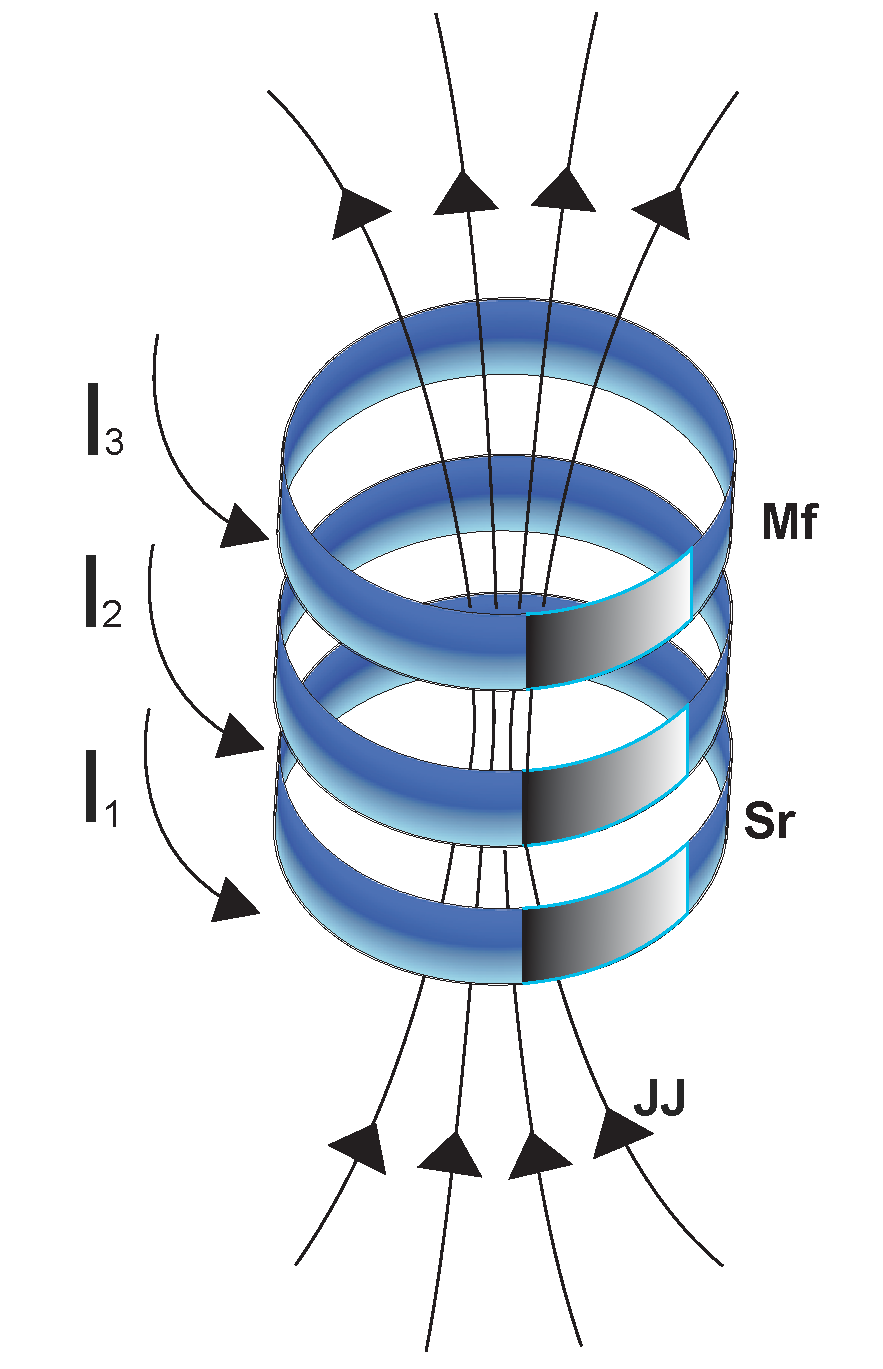
\includegraphics[scale=0.27]{Fig00}% Here is how to import EPS art
	\caption{ Schematic diagram of a SQUID trimer with  positive magnetic coupling strength,
		in a magnetic field where (Mf) is the Magnetic field, (Sr) is the Superconducting ring,
		(JJ) is the Josephson Junction, and ($I_{1}$), ($I_{2}$) and ($I_{3}$) are the induced currents.} \label{fig00}
\end{figure} 

\begin{figure*}
	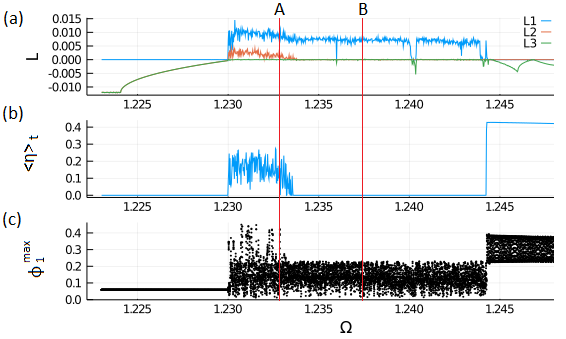
\includegraphics[scale=0.8]{Fig01}
	\caption{(a) The three maxima Lyapunov exponents (the rest are negative), (b) the mean value over time of $\eta$ and (c) maximum value of the magnetic flux $\phi_{1}$ as a function of the driving frequency. Red line A corresponds to $\Omega = 1.233$ and B to $\Omega = 1.2375$. We observe two main regions: The first one is between ($\Omega=1.23,\Omega=1.234$) corresponds to meta-stable hyper chaos synchronization where ($\left\langle \eta\right\rangle _{t} \neq 0$, $L_{1} > 0$, $L_{2} > 0$) and the second one lying between ($\Omega=1.234,\Omega=1.244$) corresponds to chaos synchronization where ($\left\langle \eta\right\rangle _{t} = 0$, $L_{1} > 0$). Parameters: $\lambda=0.1075$, $\phi_{ac}=0.02$, $\gamma=0.024$, $\phi_{dc}=0$ and $\beta=0.1369$.} \label{fig01}
\end{figure*} 

\begin{figure}
	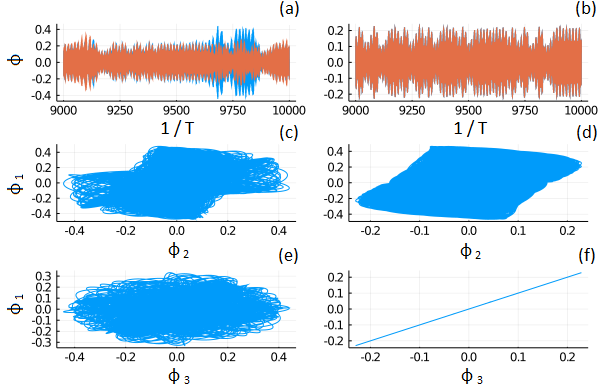
\includegraphics[scale=0.55]{Fig02}% Here is how to import EPS art
	\caption{Unsynchronized chaos for a set of parameters as in Fig. \ref{fig01} (A red line) where $ \Omega = 1.233$. (a) Time series for $\phi_{1}$ and $\phi_{3}$. (c) Projection of the flow onto $\phi_{1}$ - $\phi_{2}$ plane. (e) Projection into the $\phi_{1}$ - $\phi_{3}$ plane. (b), (d) and (f) the same for synchronized chaos where the set of parameters as in Fig. \ref{fig01} (B red line) where $\Omega = 1.2375$.} \label{fig02}
\end{figure}

\begin{figure*}
	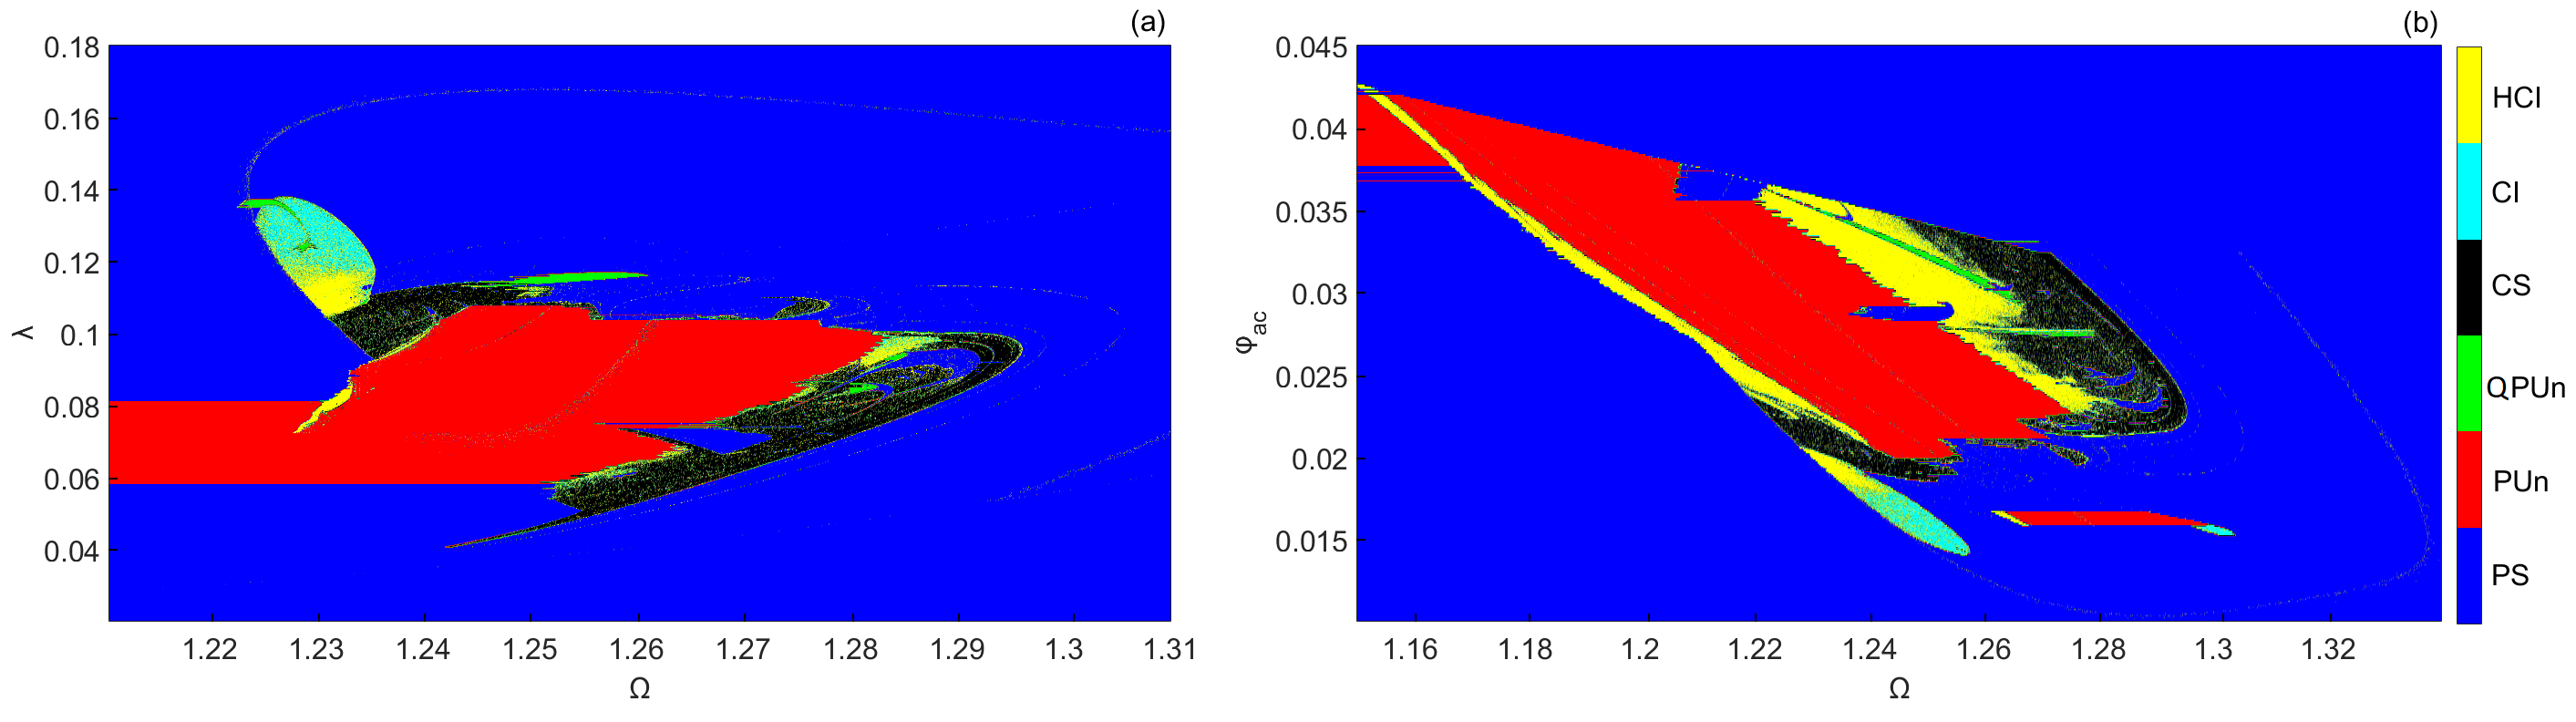
\includegraphics[scale=0.25]{Fig03}% Here is how to import EPS art
	\caption{Map of different dynamical regions in the (a) ($\lambda$,$\Omega$) parameter space where $\phi_{ac} = 0.02$ and (b) in the ($\phi_{ac}$,$\Omega$) parameter space where $\lambda = 0.02$. Depending on three maxima Lyapunov exponents ($L_{1}>L_{2}>L_{3}$) and $\left\langle \eta\right\rangle _{t}$ measurement, we observe six different areas. 
	Periodic synchronization (PS) where $L_{1}=0$ and $\left\langle \eta\right\rangle _{t} < 0.01$, Periodic unsynchronized solution (PUn)  where $L_{1}=0$ and $0.3<\left\langle \eta\right\rangle _{t}$, 
	Quasiperiodic unsynchronized solution (QPUn) where $L_{1}=L_{2}=0$ and $\left\langle \eta\right\rangle _{t} > 0.3$, 
	Chaos synchronization (CS) where $L_{1}>0,L_{2}=0$ and $\left\langle \eta\right\rangle _{t} < 0.01$, 
	Chaos intermittent synchronization (CI)  where $L_{1}>0,L_{2}=0$ and $0.01<\left\langle \eta\right\rangle _{t} < 0.3$ and finally 
	Hyperchaos intermittent synchronization (HCI)  where $L_{1}>0,L_{2}>0,L_{3}=0$ and $0.01<\left\langle \eta\right\rangle _{t} < 0.3$.} \label{fig03}
\end{figure*}

\begin{figure}
	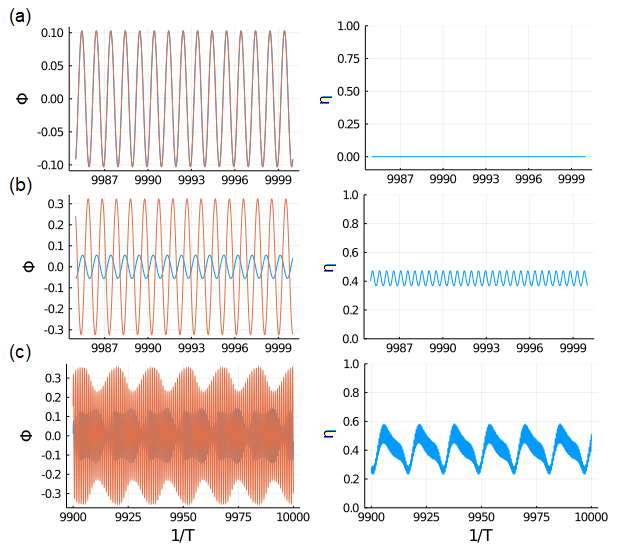
\includegraphics[scale=0.55]{Fig04_A}% Here is how to import EPS art
	\caption{(a) Periodic synchronization (PS) where $\Omega = 1.21$ and $\lambda=0.16$. (b) Periodic unsynchronized (PUn) solution where $\Omega = 1.24$ and $\lambda=0.07$ (c) Quasiperiodic unsynchronized (QPUn) solution where $\Omega = 1.255$ and $\lambda=0.118$. In first column the time series of the magnetic flux for the first SQUID, (red line), and the third SQUID, (blue line). In second column $\eta$ over time. Other parameters: $\phi_{ac}=0.02$, $\gamma=0.024$, $\phi_{dc}=0$ and $\beta=0.1369$.} \label{fig04}
\end{figure}

\begin{figure}
	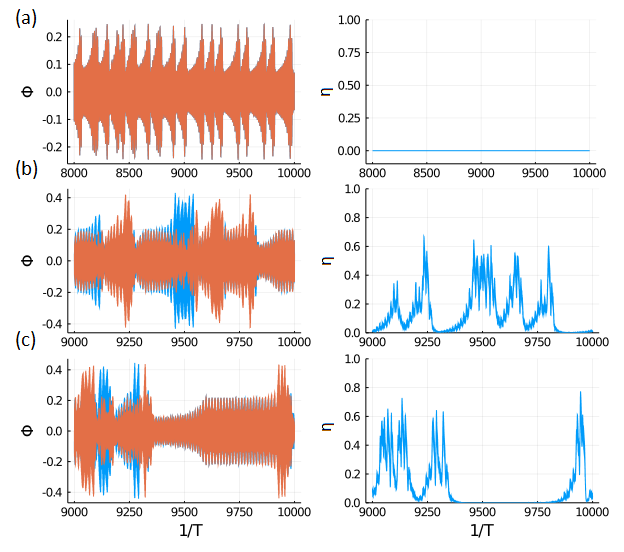
\includegraphics[scale=0.55]{Fig04_B}% Here is how to import EPS art
	\caption{(a) Chaos synchronization (CS) where $\Omega = 1.235$ and $\lambda=0.1$. (b) Chaos intermittent synchronization (CI) where $\Omega = 1.23$ and $\lambda=0.125$. (c) Hyperchaos intermittent synchronization (HCI) where $\Omega = 1.23$ and $\lambda=0.11$. First and second column as in Fig.\ref{fig04}. Other parameters: $\phi_{ac}=0.02$, $\gamma=0.024$, $\phi_{dc}=0$ and $\beta=0.1369$.} \label{fig05}
\end{figure}




%%%%%%%%%%%%%%%%%%%%%%%%%%%%%%%%%%%%%%%%%%%%%%%%%%%%%%%%%%%%%%

\section{CONCLUSIONS}\label{real}


\section{ACKNOWLEDGEMENTS}
This work was supported by the Ministry of Education and Science of the Russian Federation in the framework of the Increase Competitiveness Program of NUST ``MISiS'' (Grant number K4-2018-049).

\bibliography{bibliography}

\end{document}